\documentclass{beamer}
\usepackage{ucs}
\usepackage[utf8x]{inputenc}
\usepackage[T1]{fontenc}
\usepackage[spanish]{babel}
\usetheme{Antibes}
\setbeamercovered{transparent}
\title{"Sistema Automatizado de Ventas bajo el framework Ruby on Rails" \\ Capítulo 1}
\author{
    Bernardo Arancibia Araos
        \and Sebastián Machuca Sáez
}
\institute{
    Técnico Universitario en Informática \\ \vspace*{0.3cm}
    
\includegraphics[width=0.2\textwidth]{images/utfsm.png} \\ \vspace*{0.3cm} \tiny{Sede José Miguel Carrera} \\ 
        VIÑA DEL MAR 
}
\date{9 de Abril de 2010}

%%%%%%% DOCUMENTO %%%%%%%%%%%%%%%%%%%%

\begin{document}

\begin{frame}
\maketitle
\end{frame}

\section{Aspectos relevantes del diseño lógico}

\subsection{Descripción de la organización}

\begin{frame}
\frametitle{Descripción de la organización}
\begin{itemize}
\item \textbf{Nombre:} Provisiones Frutas y Verduras \emph{Chusmisa}
\item \textbf{Ubicación:} Población El Olivar, Viña del Mar
\item \textbf{Rubro:} Venta de Abarrotes
\end{itemize}
\end{frame}

\begin{frame}
\frametitle{Entes componentes del funcionamiento de la organización}
\begin{itemize}
\item Administrador
\item Vendedor
\item Proveedores
\end{itemize}
\end{frame}

\begin{frame}
\frametitle{Herramientas de Trabajo Actual}
\begin{itemize}
\item Balanzas Digitales
\item Refrigeradores
\item Cuadernos y hojas
\item \alert{Una Computadora}
\item \alert{Internet}
\end{itemize}
\end{frame}

\subsection{Descripción de la situación actual}

\begin{frame}
\frametitle{Descripción de la situación actual}
Se pueden identificar los siguientes procesos:
\begin{enumerate}
\item Proceso de ventas \pause                      
\item Proceso de devolución de productos \pause
\item Proceso de compra de productos mediante crédito informal \pause
\item Proceso de registro de pedidos \pause
\item Proceso de cálculo de libro de ventas \pause
\item Proceso de compra a proveedores \pause
\item Proceso de control de stock
\end{enumerate}
\end{frame}

\subsection{Problemas detectados}

\begin{frame}
\frametitle{Problemas detectados}
\begin{itemize}
\item Centralización de precios e información del negocio en una sola persona. \pause
\item No existe control de salida e ingreso de productos (stock). \pause
\item Ventas con crédito informal y pedidos se administran de forma desordenada. \pause
\item Falta de automatización en ciertas tareas.
\end{itemize}
\end{frame}


\subsection{Objetivo principal del sistema propuesto}

\begin{frame}
\begin{itemize}
\frametitle{Objetivo principal del sistema propuesto}
\item Automatizar los procesos involucrados en la gestión de venta
\end{itemize}
\end{frame}

\subsection{Descripción general del sistema propuesto}

\begin{frame}
\begin{itemize}
\frametitle{Descripción general del sistema propuesto}
\item Dos tipos de venta disponibles para el cliente. \pause
\item Registro de clientes. \pause
\item Dos formas de pago disponibles para el cliente. \pause
\item La venta culminará con el registro de ésta en la Base de Datos.
\end{itemize}
\end{frame}

\subsection{Estructura funcional del sistema propuesto}

\begin{frame}
\frametitle{Estructura funcional del sistema propuesto}
Mantenedores importantes: 
\begin{itemize}
\item Ventas
\item Clientes 
\item Pedidos 
\item Productos 
\item Créditos 
\end{itemize}
\end{frame}

\begin{frame}
Otras funcionalidades destacadas: 
\begin{itemize}
\item Control de devoluciones. \pause
\item Generar Libro de Ventas.
\end{itemize}
\end{frame}

\subsection{Entradas y Salidas}

\begin{frame}
\frametitle{Entradas y Salidas}
\begin{itemize}
\item Entradas: Datos del Producto, Cliente, Venta ... \pause
\item Salidas: Listados e informes de Productos, Ventas, Clientes ... 
\end{itemize}
\end{frame}

\subsection{Entidades de Información}

\begin{frame}
\frametitle{Entidades de Información}
\begin{enumerate}
\item Vendedores
\item Clientes
\item Proveedores
\item Productos
\item Categorías de los productos
\item Ventas 
\item Detalle de Ventas
\item Pedidos
\item Detalle de Pedidos 
\item Créditos (ventas con crédito informal)
\item Mermas  
\end{enumerate}
\end{frame}

\begin{frame}
\begin{center}
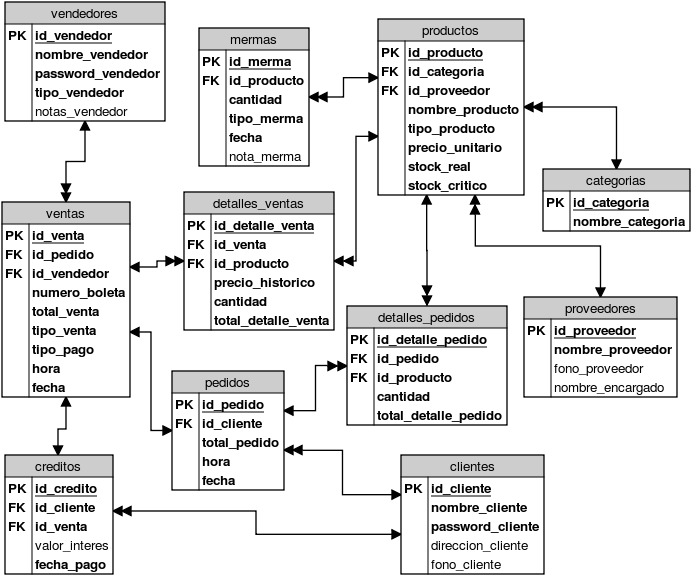
\includegraphics[width=0.8\textwidth]{images/modelo_relacional.png}
\end{center}
\end{frame}

\section{}

\begin{frame}
\frametitle{Conclusión}
\begin{center}
Identificación de Entidades para medir la magnitud del sistema a desarrollar.
\end{center}
\end{frame}

\end{document}
